%!TEX root = ../thesis.tex
\setchapterpreamble[ur][.8\textwidth]{%
\dictum[Dr. Zefram Cochrane, Entwickler des Warp-Antriebs \\ aus ``Star Trek: Enterprise – Broken Bow: Part 1'']{%
``On this site, a powerful engine will be built - an engine that will someday help us to travel a hundred times faster than we can today. [...] This engine will let us go boldly, where no man has gone before.''}
}

\chapter{WARP – Eine Webanwendung für Build- und Deployment-Prozesse}

Die Benennung einer Anwendung ist für die Entwicklung grundsätzlich irrelevant. Als Entwickler legen wir im Vorfeld trotzdem gerne einen Namen für unsere Software fest – wenigstens einen vorläufigen Projektnamen – um die Benennung verschiedenster Dinge zu erleichtern, wie Module, interne Bibliotheken, Projekte auf GitHub \& Co.

Der Projektname \textbf{WARP} wurde bei Präsentationen meist direkt mit der Science-Fiction Fernsehserie \emph{Star Trek} in Verbindung gebracht. Der Ursprung des Namens liegt jedoch nicht bei der Reise durch das All, sondern bei Nintendos Super Mario Bros.

\begin{figure}[h]
  \caption{Warp Pipes in Super Mario Bros.}
  \label{fig:super-mario-warp-pipes}
  \centering
    
\includegraphics[width=.5\textwidth]{assets/mario-pipes}
  \floatfoot{Copyright Nintendo 1985, Quelle: www.nintendo.de}
\end{figure}

Die Warp Pipes aus der Super Mario Franchise befördern unseren Pro\-ta\-go\-nisten Mario von einem Ende der Röhre an das andere Ende, welches sich weit entfernt, vielleicht auch in anderen Welten befindet. Letztendlich ist die Assoziation durch die Analogie der Rohrleitung (Pipeline) entstanden, welche auch als Begriff in Deployment-Prozessen genutzt wird.

Dieses Kapitel beinhaltet den kompletten Entwurf und die Implementierung der Anwendung WARP. Zuerst wird ein genereller Überblick über verschiedene Aspekte der Anwendung gegeben, die zum weiteren Verständnis notwendig sind. Darauf folgen Details des Services und des Clients. Da Service und Client zwei abgegrenzte Teile sind (inhaltlich und technisch), wird jeweils einzeln auf Entwurf und Implementierung eingegangen.

\section{Architekturentwurf}
\label{sec:architektur}

Die Webanwendung ist im Client-Server-Modell umgesetzt. Der Server besitzt eine API, weshalb er im weiteren Verlauf als Service bzeichnet wird (mehr dazu in \fullref{sec:service}). In folgendem Kapitel wird die grundlegende Struktur des gesamten Systems beschrieben.

\subsection{Übersicht über die Anwendung}
\label{subsec:uebersicht-anwendung}

\figref{fig:architektur} zeigt eine grafische Übersicht der Bestandteile des Systems und deren Beziehungen.

\begin{figure}[h]
  \caption{Architektur der Anwendung}
  \label{fig:architektur}
  \centering
    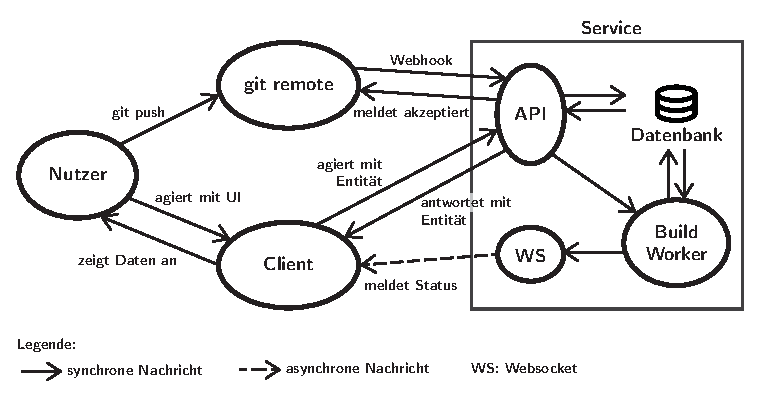
\includegraphics[width=\textwidth]{assets/systemarchitektur}
\end{figure}


Der Service ist für das Persistieren und Verwalten von Daten zuständig. Zum Abfragen und Verändern von Daten bietet der Service eine \ac{API} an. Ebenso kann der Service einen Build-Prozess starten.

Ein Build-Prozess wird gestartet, indem eine bestimmte URL über einen Git Webhook aufgerufen wird. Der Git Webhook wird so konfiguriert, dass jene URL nach jedem Push auf den Git Remote aufgerufen wird.

Der Webhook übermittelt im Body des HTTP-Requests nützliche Informationen, darunter auch Daten über den letzten Commit und die Git Reference. Mit diesen Daten kann ein passender Build-Prozess erstellt und gestartet werden.

Während des Build-Prozesses wird der aktuelle Status in Echtzeit an alle verbundenen Clients gesendet.

Der Client visualisiert letztendlich alle Daten. Über seine Oberfläche hat der Nutzer die Möglichkeit, verschiedene \ac{CRUD} Aktionen auszuführen.

\subsection{Datenstruktur}
\label{subsec:uml}

\figref{fig:uml} zeigt die Datenstruktur der Anwendung als UML Diagramm.

Die Pipeline besitzt beliebig viele Build-Prozesse als Instanzen der Pipeline. Ein solcher Build(-Prozess) ist einem Commit im Git Repository zugeordnet. Dadurch ist für den Nutzer später schneller ersichtlich, welchem Stand einem Build-Prozess zugrunde liegt.

Wie in \fullref{sec:deployment-pipeline} bereits definiert wurde, besteht eine Pipeline aus mehreren Stages, die nacheinander ausgeführt werden. In einer Stage werden Schritte oder Gruppen nacheinander (seriell) oder gleichzeitig (parallel) ausgeführt.

Eine \emph{Gruppe} ist, ähnlich wie eine Stage, eine Gruppierung von weiteren Schritten oder Gruppen, die wiederum seriell oder parallel ausgeführt werden. Gruppen lassen sich somit ineinander verschachteln, um komplexe Pipelines abbilden zu können.

Stages, Gruppen und Schritte teilen sich die gleichen Attribute. Gruppen und Schritte besitzen zusätzlich ein Attribut für den Ausführungstyp, der seriell oder parallel ist.

Ein \emph{Schritt} ist die kleinste Einheit des Build-Prozesses. Er besitzt zusätzlich Attribute für den auszuführenden Befehl und die Ausgabe (Log). Alle Schritte zusammen ergeben den gesamten Build-Prozess. Ihre Abfolge wird über die Gruppen festgelegt.

\begin{figure}[h]
  \caption{UML Diagramm der Anwendung}
  \label{fig:uml}
  \centering
    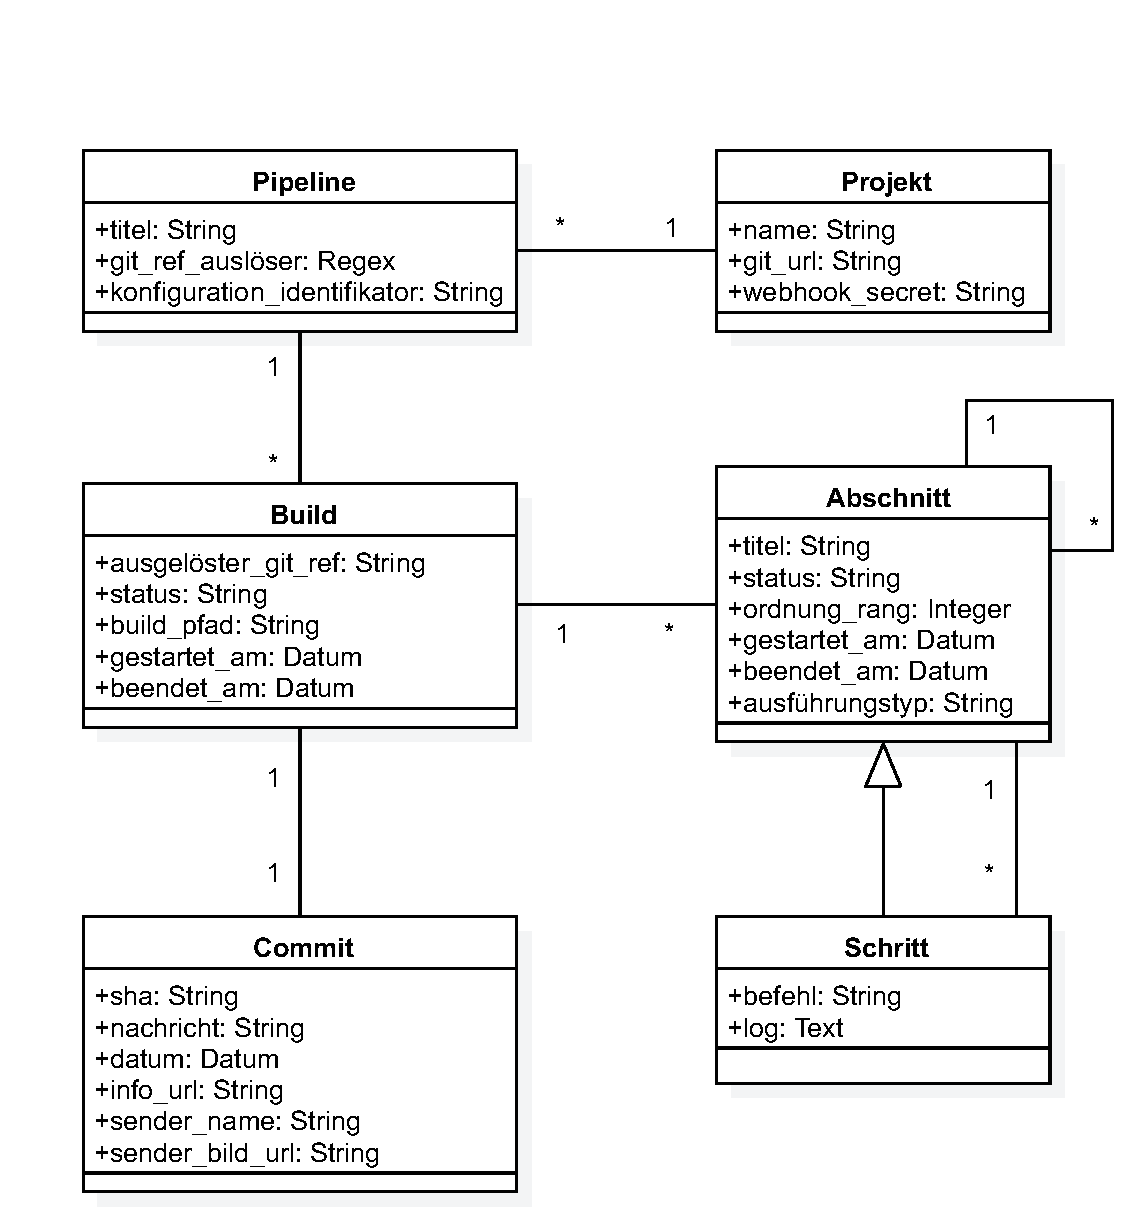
\includegraphics[width=\textwidth]{assets/uml}
\end{figure}
